% Options for packages loaded elsewhere
\PassOptionsToPackage{unicode}{hyperref}
\PassOptionsToPackage{hyphens}{url}
%
\documentclass[
]{article}
\usepackage{lmodern}
\usepackage{amssymb,amsmath}
\usepackage{ifxetex,ifluatex}
\ifnum 0\ifxetex 1\fi\ifluatex 1\fi=0 % if pdftex
  \usepackage[T1]{fontenc}
  \usepackage[utf8]{inputenc}
  \usepackage{textcomp} % provide euro and other symbols
\else % if luatex or xetex
  \usepackage{unicode-math}
  \defaultfontfeatures{Scale=MatchLowercase}
  \defaultfontfeatures[\rmfamily]{Ligatures=TeX,Scale=1}
\fi
% Use upquote if available, for straight quotes in verbatim environments
\IfFileExists{upquote.sty}{\usepackage{upquote}}{}
\IfFileExists{microtype.sty}{% use microtype if available
  \usepackage[]{microtype}
  \UseMicrotypeSet[protrusion]{basicmath} % disable protrusion for tt fonts
}{}
\makeatletter
\@ifundefined{KOMAClassName}{% if non-KOMA class
  \IfFileExists{parskip.sty}{%
    \usepackage{parskip}
  }{% else
    \setlength{\parindent}{0pt}
    \setlength{\parskip}{6pt plus 2pt minus 1pt}}
}{% if KOMA class
  \KOMAoptions{parskip=half}}
\makeatother
\usepackage{xcolor}
\IfFileExists{xurl.sty}{\usepackage{xurl}}{} % add URL line breaks if available
\IfFileExists{bookmark.sty}{\usepackage{bookmark}}{\usepackage{hyperref}}
\hypersetup{
  pdftitle={LifestyleChanges\_EmissionsAnalysis},
  pdfauthor={Zachary Palmore},
  hidelinks,
  pdfcreator={LaTeX via pandoc}}
\urlstyle{same} % disable monospaced font for URLs
\usepackage[margin=1in]{geometry}
\usepackage{color}
\usepackage{fancyvrb}
\newcommand{\VerbBar}{|}
\newcommand{\VERB}{\Verb[commandchars=\\\{\}]}
\DefineVerbatimEnvironment{Highlighting}{Verbatim}{commandchars=\\\{\}}
% Add ',fontsize=\small' for more characters per line
\usepackage{framed}
\definecolor{shadecolor}{RGB}{248,248,248}
\newenvironment{Shaded}{\begin{snugshade}}{\end{snugshade}}
\newcommand{\AlertTok}[1]{\textcolor[rgb]{0.94,0.16,0.16}{#1}}
\newcommand{\AnnotationTok}[1]{\textcolor[rgb]{0.56,0.35,0.01}{\textbf{\textit{#1}}}}
\newcommand{\AttributeTok}[1]{\textcolor[rgb]{0.77,0.63,0.00}{#1}}
\newcommand{\BaseNTok}[1]{\textcolor[rgb]{0.00,0.00,0.81}{#1}}
\newcommand{\BuiltInTok}[1]{#1}
\newcommand{\CharTok}[1]{\textcolor[rgb]{0.31,0.60,0.02}{#1}}
\newcommand{\CommentTok}[1]{\textcolor[rgb]{0.56,0.35,0.01}{\textit{#1}}}
\newcommand{\CommentVarTok}[1]{\textcolor[rgb]{0.56,0.35,0.01}{\textbf{\textit{#1}}}}
\newcommand{\ConstantTok}[1]{\textcolor[rgb]{0.00,0.00,0.00}{#1}}
\newcommand{\ControlFlowTok}[1]{\textcolor[rgb]{0.13,0.29,0.53}{\textbf{#1}}}
\newcommand{\DataTypeTok}[1]{\textcolor[rgb]{0.13,0.29,0.53}{#1}}
\newcommand{\DecValTok}[1]{\textcolor[rgb]{0.00,0.00,0.81}{#1}}
\newcommand{\DocumentationTok}[1]{\textcolor[rgb]{0.56,0.35,0.01}{\textbf{\textit{#1}}}}
\newcommand{\ErrorTok}[1]{\textcolor[rgb]{0.64,0.00,0.00}{\textbf{#1}}}
\newcommand{\ExtensionTok}[1]{#1}
\newcommand{\FloatTok}[1]{\textcolor[rgb]{0.00,0.00,0.81}{#1}}
\newcommand{\FunctionTok}[1]{\textcolor[rgb]{0.00,0.00,0.00}{#1}}
\newcommand{\ImportTok}[1]{#1}
\newcommand{\InformationTok}[1]{\textcolor[rgb]{0.56,0.35,0.01}{\textbf{\textit{#1}}}}
\newcommand{\KeywordTok}[1]{\textcolor[rgb]{0.13,0.29,0.53}{\textbf{#1}}}
\newcommand{\NormalTok}[1]{#1}
\newcommand{\OperatorTok}[1]{\textcolor[rgb]{0.81,0.36,0.00}{\textbf{#1}}}
\newcommand{\OtherTok}[1]{\textcolor[rgb]{0.56,0.35,0.01}{#1}}
\newcommand{\PreprocessorTok}[1]{\textcolor[rgb]{0.56,0.35,0.01}{\textit{#1}}}
\newcommand{\RegionMarkerTok}[1]{#1}
\newcommand{\SpecialCharTok}[1]{\textcolor[rgb]{0.00,0.00,0.00}{#1}}
\newcommand{\SpecialStringTok}[1]{\textcolor[rgb]{0.31,0.60,0.02}{#1}}
\newcommand{\StringTok}[1]{\textcolor[rgb]{0.31,0.60,0.02}{#1}}
\newcommand{\VariableTok}[1]{\textcolor[rgb]{0.00,0.00,0.00}{#1}}
\newcommand{\VerbatimStringTok}[1]{\textcolor[rgb]{0.31,0.60,0.02}{#1}}
\newcommand{\WarningTok}[1]{\textcolor[rgb]{0.56,0.35,0.01}{\textbf{\textit{#1}}}}
\usepackage{graphicx,grffile}
\makeatletter
\def\maxwidth{\ifdim\Gin@nat@width>\linewidth\linewidth\else\Gin@nat@width\fi}
\def\maxheight{\ifdim\Gin@nat@height>\textheight\textheight\else\Gin@nat@height\fi}
\makeatother
% Scale images if necessary, so that they will not overflow the page
% margins by default, and it is still possible to overwrite the defaults
% using explicit options in \includegraphics[width, height, ...]{}
\setkeys{Gin}{width=\maxwidth,height=\maxheight,keepaspectratio}
% Set default figure placement to htbp
\makeatletter
\def\fps@figure{htbp}
\makeatother
\setlength{\emergencystretch}{3em} % prevent overfull lines
\providecommand{\tightlist}{%
  \setlength{\itemsep}{0pt}\setlength{\parskip}{0pt}}
\setcounter{secnumdepth}{-\maxdimen} % remove section numbering

\title{LifestyleChanges\_EmissionsAnalysis}
\author{Zachary Palmore}
\date{11/23/2020}

\begin{document}
\maketitle

\hypertarget{abstract}{%
\subsection{Abstract}\label{abstract}}

Through data gathered from the U.S. Energy Information Administration we
found national sources of emissions have decreased significantly from
normal at 5,203.19 to an estimated 4,506.85 million metric tonnes of
carbon dioxide for the year in 2020. During this time the United States
experienced a rapid change in individual behavior due to a pandemic
caused by the SARS-CoV-2 virus. Normal emissions were calculated using
averaged data from the past 47 years where data is available. When
evaluating the significance of these reductions for agreement with the
Paris Climate Agreement, we found that further reductions must be made.

\hypertarget{introduction}{%
\subsection{Introduction}\label{introduction}}

According to the National Climate Assessment of the U.S. global change
research program, global climate is expected to continue changing, with
the magnitude of change primarily dependent on the quantity of
greenhouse gases we emit into the atmosphere (as well as how Earth's
systems respond to it). The U.S. is a significant contributor of
greenhouse gas emissions, with over 5.1 billion metric tons of carbon
dioxide (a prominent greenhouse constituent) being emitted from
energy-related sources (USGS).

Using emission data from 2010, the IPCC found that over 65\% of global
emissions come from the burning of fossil fuels in industrial processes,
including energy production. Transportation was estimated at 14\%. In
the following decade, countries have had varying levels of success in
lowering their carbon dioxide emissions by limiting the burning of
fossil fuels. Nearly all of these countries were attempting to comply
with the Paris Climate Accord. However, on November 4, 2020, the United
States formally withdrew from this agreement.

This formal withdrawal occurred in the midst of a viral pandemic that
has pushed citizens into quarantine and work-from-home arrangements, in
an attempt to quell the virus. Evidence suggests that this change in
lifestyle has influenced carbon dioxide emissions, possibly by reducing
emissions overall.

Furthermore, studies have shown that the energy consumed and produced by
sectors has shifted. According to the U.S. Energy Information
Administration, an independent energy analysis organization, energy
consumed by the residential sector increased while commercial,
transportation, and industrial sectors decreased in the same interval of
time. The largest decrease seems to have occurred in the transportation
sector with petroleum products such gasoline. These shifts in usage
reflect the change in behavior as many people were forced to work from
home, were prohibited from traveling, and reduced their vehicle usage
due to restrictions on businesses.

Since restrictions were placed by state-level governments, some have
also suggested there was a lack of coherence in messaging in those
restrictions across the nation which led many people to travel
regardless of recommendations or prohibition. This time of great pause
in daily routine traveling and switching from office sector work to
work-from-home roles should be studied. There could be underlying
benefits to this transition. One of the most worthwhile may be the
mitigation of climate change.

\hypertarget{data}{%
\subsection{Data}\label{data}}

The data in this study comes from the United State's Energy Information
Administration, an independent statistics and analysis organization. As
stated on their website, their role is ``to promote sound policymaking,
efficient markets, and public understanding of energy and its
interaction with the economy and the environment.'' This is achieved
through the review and analysis of energy-related data collected from a
combination of vetted industry and government sources. They are one of
the world's leading expert organizations in energy-related data and
provide information to a broad spectrum of consumers including federal,
state, and local governments, media, businesses, foreign governments,
research communities and the general public.

For ease of access, the data is made available through an open-source
repository on Github. It is split into three spreadsheets, each with
their own values but identical column names. To produce quality results,
some of this information needs to be reviewed alongside values of the
other spreadsheets. In simplifying the process, a fourth data frame was
created with all values combined into a single spreadsheet. This process
is explained with notes.

\begin{Shaded}
\begin{Highlighting}[]
\CommentTok{# Load the data from the remote repository}
\NormalTok{producer <-}\StringTok{ }\KeywordTok{read_csv}\NormalTok{(}\StringTok{"https://raw.githubusercontent.com/palmorezm/msdsdata607/master/Projects/Final/MER_T01_01.csv"}\NormalTok{) }
\CommentTok{# Adds energy production data}
\NormalTok{sector <-}\StringTok{ }\KeywordTok{read_csv}\NormalTok{(}\StringTok{"https://raw.githubusercontent.com/palmorezm/msdsdata607/master/Projects/Final/MER_T02_01.csv"}\NormalTok{) }
\CommentTok{# Adds energy consumption data by industry sectors}
\NormalTok{source <-}\StringTok{ }\KeywordTok{read_csv}\NormalTok{(}\StringTok{"https://raw.githubusercontent.com/palmorezm/msdsdata607/master/Projects/Final/MER_T11_01.csv"}\NormalTok{) }
\CommentTok{# Adds emissions from energy sources}


\CommentTok{# Source Cleaning}
    
    \CommentTok{# Extract monthly subsets of 2020}
\NormalTok{    source}\FloatTok{.202001}\NormalTok{ <-}\StringTok{ }\KeywordTok{subset}\NormalTok{(source, YYYYMM }\OperatorTok{==}\StringTok{ }\DecValTok{202001}\NormalTok{)}
\NormalTok{    source}\FloatTok{.202002}\NormalTok{ <-}\StringTok{ }\KeywordTok{subset}\NormalTok{(source, YYYYMM }\OperatorTok{==}\StringTok{ }\DecValTok{202002}\NormalTok{)}
\NormalTok{    source}\FloatTok{.202003}\NormalTok{ <-}\StringTok{ }\KeywordTok{subset}\NormalTok{(source, YYYYMM }\OperatorTok{==}\StringTok{ }\DecValTok{202003}\NormalTok{)}
\NormalTok{    source}\FloatTok{.202004}\NormalTok{ <-}\StringTok{ }\KeywordTok{subset}\NormalTok{(source, YYYYMM }\OperatorTok{==}\StringTok{ }\DecValTok{202004}\NormalTok{)}
\NormalTok{    source}\FloatTok{.202005}\NormalTok{ <-}\StringTok{ }\KeywordTok{subset}\NormalTok{(source, YYYYMM }\OperatorTok{==}\StringTok{ }\DecValTok{202005}\NormalTok{)}
\NormalTok{    source}\FloatTok{.202006}\NormalTok{ <-}\StringTok{ }\KeywordTok{subset}\NormalTok{(source, YYYYMM }\OperatorTok{==}\StringTok{ }\DecValTok{202006}\NormalTok{)}
\NormalTok{    source}\FloatTok{.202007}\NormalTok{ <-}\StringTok{ }\KeywordTok{subset}\NormalTok{(source, YYYYMM }\OperatorTok{==}\StringTok{ }\DecValTok{202007}\NormalTok{)}
    \CommentTok{# Combine existing monthly subsets into data frame of the partial year }
\NormalTok{    source}\FloatTok{.2020}\NormalTok{ <-}\StringTok{ }\KeywordTok{rbind}\NormalTok{(source}\FloatTok{.202001}\NormalTok{,source}\FloatTok{.202002}\NormalTok{,source}\FloatTok{.202003}\NormalTok{, source}\FloatTok{.202004}\NormalTok{,source}\FloatTok{.202005}\NormalTok{,source}\FloatTok{.202006}\NormalTok{,source}\FloatTok{.202007}\NormalTok{)}

    \CommentTok{# Order the rows by their sources and assign each value a month}
\NormalTok{    source}\FloatTok{.2020}\NormalTok{ <-}\StringTok{ }\NormalTok{source}\FloatTok{.2020} \OperatorTok\StringTok{ }
\StringTok{         }\KeywordTok{arrange}\NormalTok{(}\KeywordTok{desc}\NormalTok{(Column_Order))}
\NormalTok{    source}\FloatTok{.2020}\OperatorTok{$}\NormalTok{M <-}\StringTok{ }\KeywordTok{rep}\NormalTok{(}\KeywordTok{rep}\NormalTok{(}\DecValTok{1}\OperatorTok{:}\DecValTok{7}\NormalTok{), }\DataTypeTok{length.out =} \DecValTok{98}\NormalTok{)}
    
    \CommentTok{# Reformat dates to year-month-day}
\NormalTok{    source}\OperatorTok{$}\NormalTok{YYYYMM <-}\StringTok{ }\NormalTok{lubridate}\OperatorTok{::}\KeywordTok{parse_date_time}\NormalTok{(source}\OperatorTok{$}\NormalTok{YYYYMM, }\KeywordTok{c}\NormalTok{(}\StringTok{"ym"}\NormalTok{))}
\end{Highlighting}
\end{Shaded}

\begin{verbatim}
## Warning: 658 failed to parse.
\end{verbatim}

\begin{Shaded}
\begin{Highlighting}[]
    \CommentTok{# Extract rows that fail to parse then store as source data totals}
\NormalTok{    source.totals <-}\StringTok{ }\NormalTok{source[}\KeywordTok{rowSums}\NormalTok{(}\KeywordTok{is.na}\NormalTok{(source)) }\OperatorTok{>}\StringTok{ }\DecValTok{0}\NormalTok{,]}
    
    \CommentTok{# generate a sequence of numbers that repeats each number 14 times starting with 1973 and ending with 2020 for a total of 47 repetitions and 658 number values}
\NormalTok{    source.totals}\OperatorTok{$}\NormalTok{YYYYMM2 <-}\StringTok{ }\KeywordTok{rep}\NormalTok{(}\KeywordTok{rep}\NormalTok{(}\DecValTok{1973}\OperatorTok{:}\DecValTok{2020}\NormalTok{, }\DataTypeTok{times=}\DecValTok{47}\NormalTok{, }\DataTypeTok{each=}\DecValTok{14}\NormalTok{), }\DataTypeTok{length.out =} \DecValTok{658}\NormalTok{)}
    
    \CommentTok{# generate a sequence of numbers that repeats each number 1 time starting with 1973 and ending with 2019 for a total of 46 repetitions and 658 number values}
\NormalTok{    source.totals}\OperatorTok{$}\NormalTok{YYYYMM <-}\StringTok{ }\KeywordTok{rep}\NormalTok{(}\KeywordTok{rep}\NormalTok{(}\DecValTok{1973}\OperatorTok{:}\DecValTok{2019}\NormalTok{), }\DataTypeTok{length.out=}\DecValTok{658}\NormalTok{)}

    \CommentTok{# Extract TETCEUS monthly totals}
\NormalTok{    source.}\FloatTok{2020.}\NormalTok{totals <-}\StringTok{ }\NormalTok{source}\FloatTok{.2020} \OperatorTok
\StringTok{      }\KeywordTok{filter}\NormalTok{(MSN }\OperatorTok{==}\StringTok{ "TETCEUS"}\NormalTok{)}
  
    \CommentTok{# Compute average monthly totals of each year 1973 - 2019 using monthly observations of each year }
\NormalTok{    source.totals <-}\StringTok{ }\NormalTok{source.totals }\OperatorTok\StringTok{ }
\StringTok{      }\KeywordTok{filter}\NormalTok{(MSN }\OperatorTok{==}\StringTok{ "TETCEUS"}\NormalTok{) }\OperatorTok
\StringTok{      }\KeywordTok{mutate}\NormalTok{(}\DataTypeTok{avg_month =}\NormalTok{ Value}\OperatorTok{/}\DecValTok{12}\NormalTok{)}
    
    \CommentTok{# remove missing values from monthly source data}
\NormalTok{    source <-}\StringTok{ }\KeywordTok{na.omit}\NormalTok{(source)}
    
    
    
\CommentTok{# Producer Cleaning}
    
    \CommentTok{# Extract monthly subsets of 2020}
\NormalTok{    producer}\FloatTok{.202001}\NormalTok{ <-}\StringTok{ }\KeywordTok{subset}\NormalTok{(producer, YYYYMM }\OperatorTok{==}\StringTok{ }\DecValTok{202001}\NormalTok{)}
\NormalTok{    producer}\FloatTok{.202002}\NormalTok{ <-}\StringTok{ }\KeywordTok{subset}\NormalTok{(producer, YYYYMM }\OperatorTok{==}\StringTok{ }\DecValTok{202002}\NormalTok{)}
\NormalTok{    producer}\FloatTok{.202003}\NormalTok{ <-}\StringTok{ }\KeywordTok{subset}\NormalTok{(producer, YYYYMM }\OperatorTok{==}\StringTok{ }\DecValTok{202003}\NormalTok{)}
\NormalTok{    producer}\FloatTok{.202004}\NormalTok{ <-}\StringTok{ }\KeywordTok{subset}\NormalTok{(producer, YYYYMM }\OperatorTok{==}\StringTok{ }\DecValTok{202004}\NormalTok{)}
\NormalTok{    producer}\FloatTok{.202005}\NormalTok{ <-}\StringTok{ }\KeywordTok{subset}\NormalTok{(producer, YYYYMM }\OperatorTok{==}\StringTok{ }\DecValTok{202005}\NormalTok{)}
\NormalTok{    producer}\FloatTok{.202006}\NormalTok{ <-}\StringTok{ }\KeywordTok{subset}\NormalTok{(producer, YYYYMM }\OperatorTok{==}\StringTok{ }\DecValTok{202006}\NormalTok{)}
\NormalTok{    producer}\FloatTok{.202007}\NormalTok{ <-}\StringTok{ }\KeywordTok{subset}\NormalTok{(producer, YYYYMM }\OperatorTok{==}\StringTok{ }\DecValTok{202007}\NormalTok{)}
    \CommentTok{# Combine existing monthly subsets into data frame of the partial year }
\NormalTok{    producer}\FloatTok{.2020}\NormalTok{ <-}\StringTok{ }\KeywordTok{rbind}\NormalTok{(producer}\FloatTok{.202001}\NormalTok{,producer}\FloatTok{.202002}\NormalTok{,producer}\FloatTok{.202003}\NormalTok{, producer}\FloatTok{.202004}\NormalTok{,producer}\FloatTok{.202005}\NormalTok{,producer}\FloatTok{.202006}\NormalTok{,producer}\FloatTok{.202007}\NormalTok{)}
    
    \CommentTok{# Reformat dates to year-month-day}
\NormalTok{    producer}\OperatorTok{$}\NormalTok{YYYYMM <-}\StringTok{ }\NormalTok{lubridate}\OperatorTok{::}\KeywordTok{parse_date_time}\NormalTok{(producer}\OperatorTok{$}\NormalTok{YYYYMM, }\KeywordTok{c}\NormalTok{(}\StringTok{"ym"}\NormalTok{)) }
\end{Highlighting}
\end{Shaded}

\begin{verbatim}
## Warning: 852 failed to parse.
\end{verbatim}

\begin{Shaded}
\begin{Highlighting}[]
    \CommentTok{# Extract rows that fail to parse then store as source data totals}
\NormalTok{    producer.totals <-}\StringTok{ }\NormalTok{producer[}\KeywordTok{rowSums}\NormalTok{(}\KeywordTok{is.na}\NormalTok{(producer)) }\OperatorTok{>}\StringTok{ }\DecValTok{0}\NormalTok{,]}

  \CommentTok{# Find rows with totals prior to 1973 and reassign their dates in sequences of 23 until 12 have been completed for a total of 299 year values}
\NormalTok{  producer.pre73 <-}\StringTok{ }\NormalTok{producer.totals[}\KeywordTok{c}\NormalTok{(}\DecValTok{1}\OperatorTok{:}\DecValTok{24}\NormalTok{, }\DecValTok{72}\OperatorTok{:}\DecValTok{96}\NormalTok{, }\DecValTok{143}\OperatorTok{:}\DecValTok{167}\NormalTok{, }\DecValTok{214}\OperatorTok{:}\DecValTok{238}\NormalTok{, }\DecValTok{285}\OperatorTok{:}\DecValTok{309}\NormalTok{, }\DecValTok{356}\OperatorTok{:}\DecValTok{380}\NormalTok{, }\DecValTok{427}\OperatorTok{:}\DecValTok{451}\NormalTok{, }\DecValTok{498}\OperatorTok{:}\DecValTok{522}\NormalTok{, }\DecValTok{569}\OperatorTok{:}\DecValTok{593}\NormalTok{, }\DecValTok{640}\OperatorTok{:}\DecValTok{664}\NormalTok{, }\DecValTok{711}\OperatorTok{:}\DecValTok{735}\NormalTok{, }\DecValTok{782}\OperatorTok{:}\DecValTok{806}\NormalTok{),]}
\NormalTok{  producer.pre73}\OperatorTok{$}\NormalTok{YYYYMM <-}\StringTok{ }\KeywordTok{rep}\NormalTok{(}\KeywordTok{rep}\NormalTok{(}\DecValTok{1949}\OperatorTok{:}\DecValTok{1972}\NormalTok{), }\DataTypeTok{length.out =} \DecValTok{299}\NormalTok{)}
  
    \CommentTok{# Using 1973+ apply the sequence generation as yyyy-mm-dd to producers; repeat 1973 - 2019   }
\NormalTok{  producer.totals <-}\StringTok{  }\NormalTok{producer.totals[}\KeywordTok{c}\NormalTok{(}\DecValTok{25}\OperatorTok{:}\DecValTok{71}\NormalTok{,}\DecValTok{97}\OperatorTok{:}\DecValTok{142}\NormalTok{,}\DecValTok{168}\OperatorTok{:}\DecValTok{213}\NormalTok{, }\DecValTok{239}\OperatorTok{:}\DecValTok{284}\NormalTok{,}\DecValTok{310}\OperatorTok{:}\DecValTok{355}\NormalTok{, }\DecValTok{381}\OperatorTok{:}\DecValTok{426}\NormalTok{, }\DecValTok{452}\OperatorTok{:}\DecValTok{497}\NormalTok{, }\DecValTok{523}\OperatorTok{:}\DecValTok{568}\NormalTok{, }\DecValTok{594}\OperatorTok{:}\DecValTok{639}\NormalTok{, }\DecValTok{665}\OperatorTok{:}\DecValTok{710}\NormalTok{, }\DecValTok{736}\OperatorTok{:}\DecValTok{781}\NormalTok{, }\DecValTok{807}\OperatorTok{:}\DecValTok{852}\NormalTok{),]}
  
  
  \CommentTok{# remove missing values from monthly source data}
\NormalTok{  producer <-}\StringTok{  }\KeywordTok{na.omit}\NormalTok{(producer)}
  
  
  
\CommentTok{# Sector Cleaning}
    
     \CommentTok{# Reformat dates to year-month-day}
\NormalTok{    sector}\OperatorTok{$}\NormalTok{YYYYMM <-}\StringTok{ }\NormalTok{lubridate}\OperatorTok{::}\KeywordTok{parse_date_time}\NormalTok{(sector}\OperatorTok{$}\NormalTok{YYYYMM, }\KeywordTok{c}\NormalTok{(}\StringTok{"ym"}\NormalTok{)) }
\end{Highlighting}
\end{Shaded}

\begin{verbatim}
## Warning: 781 failed to parse.
\end{verbatim}

\begin{Shaded}
\begin{Highlighting}[]
    \CommentTok{# Extract rows that fail to parse then store as source data totals}
\NormalTok{    sector.totals <-}\StringTok{ }\NormalTok{sector[}\KeywordTok{rowSums}\NormalTok{(}\KeywordTok{is.na}\NormalTok{(sector)) }\OperatorTok{>}\StringTok{ }\DecValTok{0}\NormalTok{,]}

\CommentTok{# Combine sources into one data frame}
\NormalTok{all <-}\StringTok{ }\KeywordTok{rbind}\NormalTok{(producer, sector, source) }
\end{Highlighting}
\end{Shaded}

A subset of the source data set is shown below. Carbon dioxide emissions
from sources data set will be the primary data frame to perform
calculations and work from. Excluding the combined \emph{all} data,
other data frames, will not contain emissions statistics as their
durations and interations of data collection differ from one another and
it is not necessary to extend this study further into the past.
Retroactive studies have been completed before, our focus is on the
change in levels of carbon dioxide for the year 2020 from the past
nearly half-century's trends in emissions to determine its significance
and potential implications.

\begin{Shaded}
\begin{Highlighting}[]
\NormalTok{source[}\DecValTok{1}\OperatorTok{:}\DecValTok{4}\NormalTok{, }\KeywordTok{c}\NormalTok{(}\DecValTok{1}\OperatorTok{:}\DecValTok{3}\NormalTok{,}\DecValTok{5}\NormalTok{)]}
\end{Highlighting}
\end{Shaded}

\begin{verbatim}
## # A tibble: 4 x 4
##   MSN     YYYYMM              Value Description                                 
##   <chr>   <dttm>              <dbl> <chr>                                       
## 1 CKTCEUS 1973-01-01 00:00:00 108.  Coal, Including Coal Coke Net Imports, CO2 ~
## 2 CKTCEUS 1973-02-01 00:00:00  97.7 Coal, Including Coal Coke Net Imports, CO2 ~
## 3 CKTCEUS 1973-03-01 00:00:00  97.3 Coal, Including Coal Coke Net Imports, CO2 ~
## 4 CKTCEUS 1973-04-01 00:00:00  93.1 Coal, Including Coal Coke Net Imports, CO2 ~
\end{verbatim}

This data frame displays the carbon dioxide emissions by source. There
are 7,994 observations of 6 variable types. The columns for
\emph{Column\_Order} and \emph{Unit} have been removed as they are not
necessary for display. They are, however, useful for calculations,
munging, and filtering through vast swaths of this data. For our
purposes, they remain hidden in the table.

Only the first 4 rows are shown. This is just enough demonstrate
variation in the column labeled \emph{Value} which is the amount of
emissions. These are measured in units of a million metric tons of
carbon dioxide equivalent or mttco2e. Each column has its own key.
Column name \emph{MSN} in the unique identifier of source names and
stands for mnemonic series names. Column \emph{YYYYMM} provides the date
in a date formatted with lubridate. Since they were not provided, all
days were selected to the first two-digit day of the four-digit year and
2-digit month respectively. Lastly, the \emph{Description} column
supplies the unique identifier of source names in long-form for
reference.

The combined data set \emph{all} contains the values of energy producers
and their production amount, emission sources and their total emissions
of carbon dioxide, and the sectors energy flows through as well as the
quantities consumed by those sectors. These are broken out further into
subsections of the data since there are 21,908 observations of those
same 6 variables across all the data in this data set.

\hypertarget{analysis}{%
\subsection{Analysis}\label{analysis}}

With clean data, we start by finding the averages of the total amount of
carbon dioxide emissions from U.S. sources in our study year and over
the duration of the study. We use emissions data spanning 1973 to 2019
to determine the normal level of emissions using a mean of sums where
data was available. The average of 2020 was calculated by finding the
mean of all available months within the year. This is our study year and
it contains 7 values of total emissions by source beginning in January
and running consecutively through the year by month. The calculation
process is documented below.

\begin{Shaded}
\begin{Highlighting}[]
\CommentTok{# Mean CO2 since 1973 - given reliable source data}
\NormalTok{normal.co2 <-}\StringTok{ }\NormalTok{source.totals }\OperatorTok\StringTok{ }
\StringTok{  }\KeywordTok{filter}\NormalTok{(Column_Order }\OperatorTok{==}\StringTok{ }\DecValTok{14}\NormalTok{) }\OperatorTok\StringTok{ }
\StringTok{  }\KeywordTok{summarise}\NormalTok{(}\DataTypeTok{since_1973 =} \KeywordTok{mean}\NormalTok{(Value))}

\CommentTok{# Total co2 in 2020 thus far}
\NormalTok{thusfar}\FloatTok{.2020}\NormalTok{ <-}\StringTok{ }\NormalTok{source}\FloatTok{.2020} \OperatorTok\StringTok{ }
\StringTok{  }\KeywordTok{filter}\NormalTok{(Column_Order }\OperatorTok{==}\StringTok{ }\DecValTok{14}\NormalTok{) }\OperatorTok\StringTok{ }
\StringTok{  }\KeywordTok{summarise}\NormalTok{(}\DataTypeTok{thusfar.2020 =} \KeywordTok{sum}\NormalTok{(Value)) }
  
\CommentTok{# Mean of co2 thus far in 2020}
\NormalTok{thusfar.}\FloatTok{2020.}\NormalTok{mean <-}\StringTok{ }\NormalTok{source}\FloatTok{.2020} \OperatorTok
\StringTok{  }\KeywordTok{filter}\NormalTok{(Column_Order }\OperatorTok{==}\StringTok{ }\DecValTok{14}\NormalTok{) }\OperatorTok
\StringTok{  }\KeywordTok{summarise}\NormalTok{(}\DataTypeTok{mean =} \KeywordTok{mean}\NormalTok{(Value))}

\CommentTok{# Find expected co2 with current mean emissions for year}
\NormalTok{est.co2 <-}\StringTok{ }\KeywordTok{signif}\NormalTok{(thusfar}\FloatTok{.2020} \OperatorTok{+}\StringTok{ }\NormalTok{(thusfar.}\FloatTok{2020.}\NormalTok{mean }\OperatorTok{*}\StringTok{ }\DecValTok{5}\NormalTok{), }\DataTypeTok{digits =} \DecValTok{6}\NormalTok{)}
                  
\NormalTok{est.co2 <-}\StringTok{ }\KeywordTok{data_frame}\NormalTok{(normal.co2, est.co2) }\OperatorTok\StringTok{ }
\StringTok{  }\KeywordTok{mutate}\NormalTok{(}\DataTypeTok{dif =}\NormalTok{ since_}\DecValTok{1973} \OperatorTok{-}\StringTok{ }\NormalTok{thusfar}\FloatTok{.2020}\NormalTok{) }\OperatorTok\StringTok{ }
\StringTok{  }\KeywordTok{rename}\NormalTok{(}\DataTypeTok{est.2020 =}\NormalTok{ thusfar}\FloatTok{.2020}\NormalTok{,}
         \DataTypeTok{obs.1973 =}\NormalTok{ since_}\DecValTok{1973}\NormalTok{) }
\end{Highlighting}
\end{Shaded}

\begin{verbatim}
## Warning: `data_frame()` is deprecated as of tibble 1.1.0.
## Please use `tibble()` instead.
## This warning is displayed once every 8 hours.
## Call `lifecycle::last_warnings()` to see where this warning was generated.
\end{verbatim}

\begin{Shaded}
\begin{Highlighting}[]
\CommentTok{# Change calculation values to numeric values outside the data frame}
\NormalTok{totalco2}\FloatTok{.2020}\NormalTok{ <-}\StringTok{ }\KeywordTok{round}\NormalTok{(thusfar}\FloatTok{.2020}\OperatorTok{$}\NormalTok{thusfar}\FloatTok{.2020}\NormalTok{, }\DataTypeTok{digits=} \DecValTok{2}\NormalTok{)}
\NormalTok{meanco2}\FloatTok{.2020}\NormalTok{ <-}\StringTok{ }\KeywordTok{round}\NormalTok{(thusfar.}\FloatTok{2020.}\NormalTok{mean}\OperatorTok{$}\NormalTok{mean, }\DataTypeTok{digits =} \DecValTok{2}\NormalTok{)}

\CommentTok{# Differences as a proportion and percentage }
\NormalTok{Peo <-}\StringTok{ }\KeywordTok{signif}\NormalTok{((est.co2}\OperatorTok{$}\NormalTok{est}\FloatTok{.2020}\OperatorTok{/}\NormalTok{est.co2}\OperatorTok{$}\NormalTok{obs}\FloatTok{.1973}\NormalTok{), }\DataTypeTok{digits =} \DecValTok{4}\NormalTok{)}
\NormalTok{Peo.dif <-}\StringTok{ }\KeywordTok{signif}\NormalTok{((est.co2}\OperatorTok{$}\NormalTok{obs}\FloatTok{.1973} \OperatorTok{-}\StringTok{ }\NormalTok{est.co2}\OperatorTok{$}\NormalTok{est}\FloatTok{.2020}\NormalTok{)}\OperatorTok{/}\NormalTok{(est.co2}\OperatorTok{$}\NormalTok{obs}\FloatTok{.1973}\NormalTok{), }\DataTypeTok{digits =} \DecValTok{4}\NormalTok{)}
\NormalTok{reduction}\FloatTok{.2020}\NormalTok{ <-}\StringTok{ }\KeywordTok{signif}\NormalTok{((Peo }\OperatorTok{-}\StringTok{ }\NormalTok{Peo.dif), }\DataTypeTok{digits =} \DecValTok{4}\NormalTok{)}
\end{Highlighting}
\end{Shaded}

Total carbon dioxide emissions from January through July of 2020 is
2628.99 million metric tons of carbon dioxide equivalent (mmtco2e). The
average monthly amount of emissions from all energy sources is 375.57
mmtco2e. This is quantified by calculating the sum of total emission
sources from January through July of 2020. If emissions are close to the
average for the remaining five months (August through December) then the
total emissions of the U.S. energy sources for the year would be about
4506.85 mmtco2e. The average amount of total emissions from 1973 to 2019
is 4506.85 mmtco2e.

Emissions for all completed years are plotted as a scatterplot in figure
1 showing the trends in emissions since 1973. A locally weighted
scatterplot smoothing (loess) line was computed along with the points to
normalize the pattern. In blue, the dashed line represents the average
amount of total emissions under normal conditions in this study. In dark
green, the dot-dashed line is the potential total emissions for the year
2020 if emissions remained at the average level of the first 7 months.
All emissions quantities are measured in million metric tons of carbon
dioxide equivalent (mmtco2e).

\begin{Shaded}
\begin{Highlighting}[]
\NormalTok{source.totals }\OperatorTok\StringTok{ }
\StringTok{  }\KeywordTok{filter}\NormalTok{(Description }\OperatorTok{==}\StringTok{ "Total Energy CO2 Emissions"}\NormalTok{) }\OperatorTok\StringTok{ }
\StringTok{  }\KeywordTok{ggplot}\NormalTok{(}\KeywordTok{aes}\NormalTok{(YYYYMM, Value)) }\OperatorTok{+}\StringTok{ }
\StringTok{  }\KeywordTok{geom_point}\NormalTok{(}\KeywordTok{aes}\NormalTok{(}\DataTypeTok{color =}\NormalTok{ Description)) }\OperatorTok{+}\StringTok{ }
\StringTok{  }\KeywordTok{geom_smooth}\NormalTok{() }\OperatorTok{+}\StringTok{ }
\StringTok{  }\KeywordTok{geom_hline}\NormalTok{(}\DataTypeTok{yintercept =}\NormalTok{ est.co2}\OperatorTok{$}\NormalTok{obs}\FloatTok{.1973}\NormalTok{, }\DataTypeTok{color =} \StringTok{"blue"}\NormalTok{, }\DataTypeTok{linetype =} \StringTok{"dashed"}\NormalTok{)  }\OperatorTok{+}
\StringTok{  }\KeywordTok{geom_hline}\NormalTok{(}\DataTypeTok{yintercept =}\NormalTok{ est.co2}\OperatorTok{$}\NormalTok{est}\FloatTok{.2020}\NormalTok{, }\DataTypeTok{color =} \StringTok{"dark green"}\NormalTok{, }\DataTypeTok{linetype =} \StringTok{"dotdash"}\NormalTok{, }\DataTypeTok{size =} \DecValTok{1}\NormalTok{) }\OperatorTok{+}
\StringTok{    }\KeywordTok{labs}\NormalTok{(}\DataTypeTok{x =} \StringTok{"Time"}\NormalTok{, }
       \DataTypeTok{y =} \StringTok{"Million Metric Tons CO2"}\NormalTok{, }
       \DataTypeTok{title =} \StringTok{"Total CO2 Emissions in US"}\NormalTok{, }
       \DataTypeTok{subtitle =} \StringTok{"Using Yearly Totals from All Energy Sources"}\NormalTok{, }
       \DataTypeTok{caption =} \StringTok{"Figure 1"}\NormalTok{) }\OperatorTok{+}\StringTok{ }
\StringTok{  }\KeywordTok{theme_classic}\NormalTok{() }\OperatorTok{+}\StringTok{ }
\StringTok{  }\KeywordTok{theme}\NormalTok{(}\DataTypeTok{plot.title =} \KeywordTok{element_text}\NormalTok{(}\DataTypeTok{hjust =} \FloatTok{0.5}\NormalTok{),}
        \DataTypeTok{plot.subtitle =} \KeywordTok{element_text}\NormalTok{(}\DataTypeTok{hjust =} \FloatTok{0.5}\NormalTok{), }
        \DataTypeTok{legend.position =} \StringTok{"none"}\NormalTok{,}
        \DataTypeTok{plot.caption =} \KeywordTok{element_text}\NormalTok{(}\DataTypeTok{hjust =} \FloatTok{0.5}\NormalTok{))}
\end{Highlighting}
\end{Shaded}

\begin{verbatim}
## `geom_smooth()` using method = 'loess' and formula 'y ~ x'
\end{verbatim}

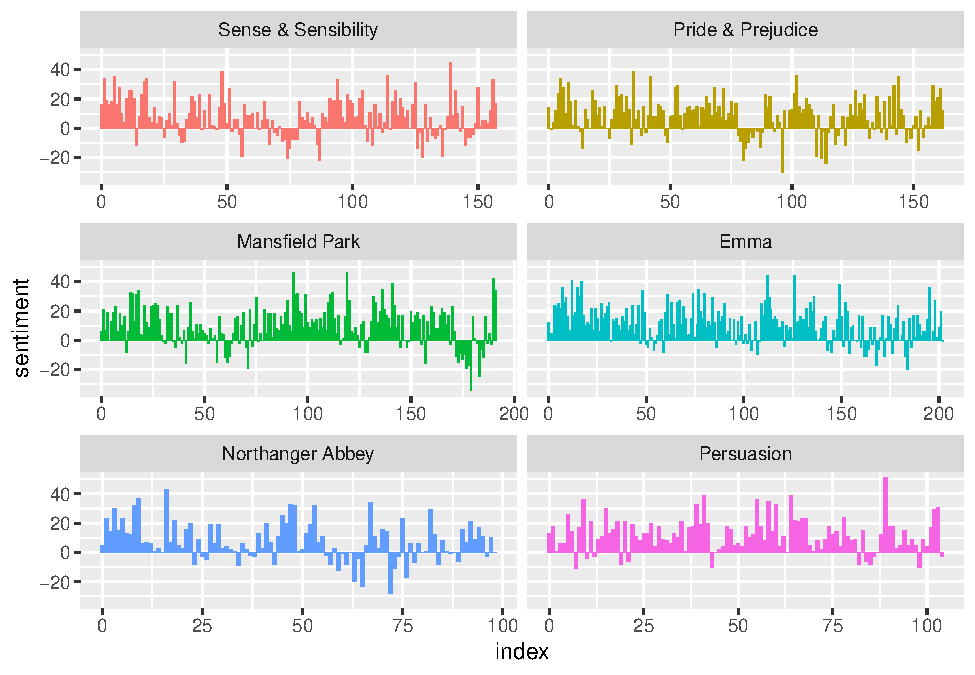
\includegraphics{Final_Project_files/figure-latex/unnamed-chunk-4-1.pdf}

We notice the emissions line for our study year is below the normal
(dashed) emissions line for the entirety of the study duration. Since
the calculation for our study year only contains the first 7 months,
this is only an estimate. However, if new monthly conditions were to
remain at or near the average for the months of January through July of
2020 then average emissions could decrease from normal by approximately
696.3399787 mmtco2e. That is a reduction in emissions of about 73.24\%
from normal.

In furthering this scenario, we determine whether these variables have a
strong correlation and if this reduction would be a significant
deviation from natural variation. For this, we perform a Welch Two
Sample t-test to compare the average monthly totals from the years 1973
through 2019 with observations of the monthly totals from 2020. We also
conduct a Pearson's product-moment correlation on the observations of
total emissions related to each year and use a linear model to evaluate
the average monthly observations of 2020. Additionally, we compute 95\%
confidence intervals on the monthly observations for the study year and
the data from what we considered the normal range.

\begin{Shaded}
\begin{Highlighting}[]
\NormalTok{t <-}\StringTok{ }\FloatTok{1.96} \CommentTok{# at 95% confidence }
\CommentTok{# source.yyyy indicates the start year}
\NormalTok{x.source2020 <-}\StringTok{ }\KeywordTok{mean}\NormalTok{(source.}\FloatTok{2020.}\NormalTok{totals}\OperatorTok{$}\NormalTok{Value, }\DataTypeTok{na.rm =} \OtherTok{TRUE}\NormalTok{)}
\NormalTok{sd.source2020 <-}\StringTok{  }\KeywordTok{sd}\NormalTok{(source.}\FloatTok{2020.}\NormalTok{totals}\OperatorTok{$}\NormalTok{Value, }\DataTypeTok{na.rm =} \OtherTok{TRUE}\NormalTok{)}
\NormalTok{n.source2020 <-}\StringTok{ }\NormalTok{source.}\FloatTok{2020.}\NormalTok{totals }\OperatorTok
\StringTok{  }\KeywordTok{summarise}\NormalTok{(}\DataTypeTok{freq =} \KeywordTok{table}\NormalTok{(Value)) }\OperatorTok
\StringTok{  }\KeywordTok{summarise}\NormalTok{(}\DataTypeTok{n =} \KeywordTok{sum}\NormalTok{(freq, }\DataTypeTok{na.rm =} \OtherTok{TRUE}\NormalTok{))}
\NormalTok{upper.ci}\FloatTok{.2020}\NormalTok{ <-}\StringTok{ }\NormalTok{x.source2020 }\OperatorTok{+}\StringTok{ }\NormalTok{t}\OperatorTok{*}\NormalTok{(sd.source2020}\OperatorTok{/}\KeywordTok{sqrt}\NormalTok{(n.source2020}\OperatorTok{$}\NormalTok{n))}
\NormalTok{lower.ci}\FloatTok{.2020}\NormalTok{ <-}\StringTok{ }\NormalTok{x.source2020 }\OperatorTok{-}\StringTok{ }\NormalTok{t}\OperatorTok{*}\NormalTok{(sd.source2020}\OperatorTok{/}\KeywordTok{sqrt}\NormalTok{(n.source2020}\OperatorTok{$}\NormalTok{n))}
\CommentTok{# interval for 1973 to 2019}
\NormalTok{x.source1973 <-}\StringTok{ }\KeywordTok{mean}\NormalTok{(source.totals}\OperatorTok{$}\NormalTok{avg_month, }\DataTypeTok{na.rm =} \OtherTok{TRUE}\NormalTok{)}
\NormalTok{sd.source1973 <-}\StringTok{  }\KeywordTok{sd}\NormalTok{(source.totals}\OperatorTok{$}\NormalTok{avg_month, }\DataTypeTok{na.rm =} \OtherTok{TRUE}\NormalTok{)}
\NormalTok{n.source1973 <-}\StringTok{ }\NormalTok{source.totals }\OperatorTok
\StringTok{  }\KeywordTok{summarise}\NormalTok{(}\DataTypeTok{freq =} \KeywordTok{table}\NormalTok{(avg_month)) }\OperatorTok
\StringTok{  }\KeywordTok{summarise}\NormalTok{(}\DataTypeTok{n =} \KeywordTok{sum}\NormalTok{(freq, }\DataTypeTok{na.rm =} \OtherTok{TRUE}\NormalTok{))}
\NormalTok{upper.ci}\FloatTok{.1973}\NormalTok{ <-}\StringTok{ }\NormalTok{x.source1973 }\OperatorTok{+}\StringTok{ }\NormalTok{t}\OperatorTok{*}\NormalTok{(sd.source1973}\OperatorTok{/}\KeywordTok{sqrt}\NormalTok{(n.source1973}\OperatorTok{$}\NormalTok{n))}
\NormalTok{lower.ci}\FloatTok{.1973}\NormalTok{ <-}\StringTok{ }\NormalTok{x.source1973 }\OperatorTok{-}\StringTok{ }\NormalTok{t}\OperatorTok{*}\NormalTok{(sd.source1973}\OperatorTok{/}\KeywordTok{sqrt}\NormalTok{(n.source1973}\OperatorTok{$}\NormalTok{n))}
\NormalTok{cor.test <-}\StringTok{ }\KeywordTok{cor.test}\NormalTok{(source.totals}\OperatorTok{$}\NormalTok{Value, source.totals}\OperatorTok{$}\NormalTok{YYYYMM)}
\NormalTok{co2.lm <-}\StringTok{ }\KeywordTok{lm}\NormalTok{(source.totals}\OperatorTok{$}\NormalTok{YYYYMM }\OperatorTok{~}\StringTok{ }\NormalTok{source.totals}\OperatorTok{$}\NormalTok{avg_month)}
\NormalTok{co2.lm.res <-}\StringTok{ }\KeywordTok{summary}\NormalTok{(co2.lm)}
\NormalTok{t.test <-}\StringTok{ }\KeywordTok{t.test}\NormalTok{(source.}\FloatTok{2020.}\NormalTok{totals}\OperatorTok{$}\NormalTok{Value, source.totals}\OperatorTok{$}\NormalTok{avg_month)}
\end{Highlighting}
\end{Shaded}

From the Welch Two Sample t-test we find the results are significant at
an alpha level of 0.05 with a p-value of 0.0269096. We should reject the
null hypothesis in favor of our alternative that there is a significant
difference in the mean of monthly carbon dioxide emissions in the year
2020. We are 95\% confident that the true mean of emissions in the study
year must be between 336.3540776 and 414.7870652. We are also 95\%
confident that the true mean of emissions in the study duration is
between 422.2298898 and 444.96844 which favors the results of this
hypothesis test.

Results from the Pearson's product-moment test indicate a moderately
strong positive relationship of total emissions each year with a
correlation value of 0.687. We have great confidence in the year as a
predictor of total emissions with a t-value of 6.34.

Our linear regression model produced a slightly positive linear
association and confirmed the results of the product-moment test
producing a t-value of 6.34. This indicates strength in our coefficient,
in this case measured in months, as a predictor of the total average
emissions. We also confirmed the Welch Two Sample t-test conclusion that
we should reject the null hypothesis in favor of the alternative given
our p-value of \ensuremath{9.9\times 10^{-8}}. The variation in total
carbon dioxide emission in 2020 is highly unlikely to have occurred by
random chance. The formula for this model is as follows:

\[ f(x) = 0.2368(x) + 1893.3383\]

However, the coefficients of determination for this linear model were
moderately weak with an r-squared of 0.472 and an adjusted r-squared of
0.46. These measure the proportion of variation in our average monthly
emissions as a factor caused by the unit of time, months. Given that
every month has a near perfect sequence and near zero variation, these
results are surprising and reasonable. It indicates the total average
monthly emissions from carbon dioxide have grown fairly steadily from
1973 to 2019 without much variation. But, there is likely a better model
to fit this data. Note that these results do not include those of 2020
to support more robust statistics.

Extending this analysis, variation in emissions totals from all energy
sources can be shown as a similar scatterplot to the one shown in figure
1. However, this takes the data and breaks it down further by month.
Observe the trend in figure 2 below. Here again the dot-dash green line
shows the average (mean) monthly emissions in 2020 and the dashed blue
represents the average (mean) monthly emissions from 1973 through 2019.

\begin{Shaded}
\begin{Highlighting}[]
\NormalTok{source }\OperatorTok\StringTok{ }
\StringTok{  }\KeywordTok{filter}\NormalTok{(Column_Order }\OperatorTok{==}\StringTok{ }\DecValTok{14}\NormalTok{) }\OperatorTok\StringTok{ }
\StringTok{  }\KeywordTok{ggplot}\NormalTok{(}\KeywordTok{aes}\NormalTok{(YYYYMM, Value)) }\OperatorTok{+}\StringTok{ }
\StringTok{  }\KeywordTok{geom_point}\NormalTok{(}\KeywordTok{aes}\NormalTok{(}\DataTypeTok{color =}\NormalTok{ Description)) }\OperatorTok{+}\StringTok{ }
\StringTok{  }\KeywordTok{geom_smooth}\NormalTok{() }\OperatorTok{+}\StringTok{ }
\StringTok{  }\KeywordTok{geom_hline}\NormalTok{(}\DataTypeTok{yintercept =}\NormalTok{ est.co2}\OperatorTok{$}\NormalTok{obs}\FloatTok{.1973}\OperatorTok{/}\DecValTok{12}\NormalTok{, }\DataTypeTok{color =} \StringTok{"blue"}\NormalTok{, }\DataTypeTok{linetype =} \StringTok{"dashed"}\NormalTok{)  }\OperatorTok{+}
\StringTok{  }\KeywordTok{geom_hline}\NormalTok{(}\DataTypeTok{yintercept =}\NormalTok{ est.co2}\OperatorTok{$}\NormalTok{est}\FloatTok{.2020}\OperatorTok{/}\DecValTok{12}\NormalTok{, }\DataTypeTok{color =} \StringTok{"dark green"}\NormalTok{, }\DataTypeTok{linetype =} \StringTok{"dotdash"}\NormalTok{, }\DataTypeTok{size =} \DecValTok{1}\NormalTok{) }\OperatorTok{+}
\StringTok{    }\KeywordTok{labs}\NormalTok{(}\DataTypeTok{x =} \StringTok{"Time"}\NormalTok{, }
       \DataTypeTok{y =} \StringTok{"Million Metric Tons CO2"}\NormalTok{, }
       \DataTypeTok{title =} \StringTok{"Total CO2 Emissions in US"}\NormalTok{, }
       \DataTypeTok{subtitle =} \StringTok{"Using Monthly Totals from All Energy Sources"}\NormalTok{, }
       \DataTypeTok{caption =} \StringTok{"Figure 2"}\NormalTok{) }\OperatorTok{+}\StringTok{ }
\StringTok{  }\KeywordTok{theme_classic}\NormalTok{() }\OperatorTok{+}\StringTok{ }
\StringTok{  }\KeywordTok{theme}\NormalTok{(}\DataTypeTok{plot.title =} \KeywordTok{element_text}\NormalTok{(}\DataTypeTok{hjust =} \FloatTok{0.5}\NormalTok{),}
        \DataTypeTok{plot.subtitle =} \KeywordTok{element_text}\NormalTok{(}\DataTypeTok{hjust =} \FloatTok{0.5}\NormalTok{), }
        \DataTypeTok{legend.position =} \StringTok{"none"}\NormalTok{,}
        \DataTypeTok{plot.caption =} \KeywordTok{element_text}\NormalTok{(}\DataTypeTok{hjust =} \FloatTok{0.5}\NormalTok{))}
\end{Highlighting}
\end{Shaded}

\begin{verbatim}
## `geom_smooth()` using method = 'loess' and formula 'y ~ x'
\end{verbatim}

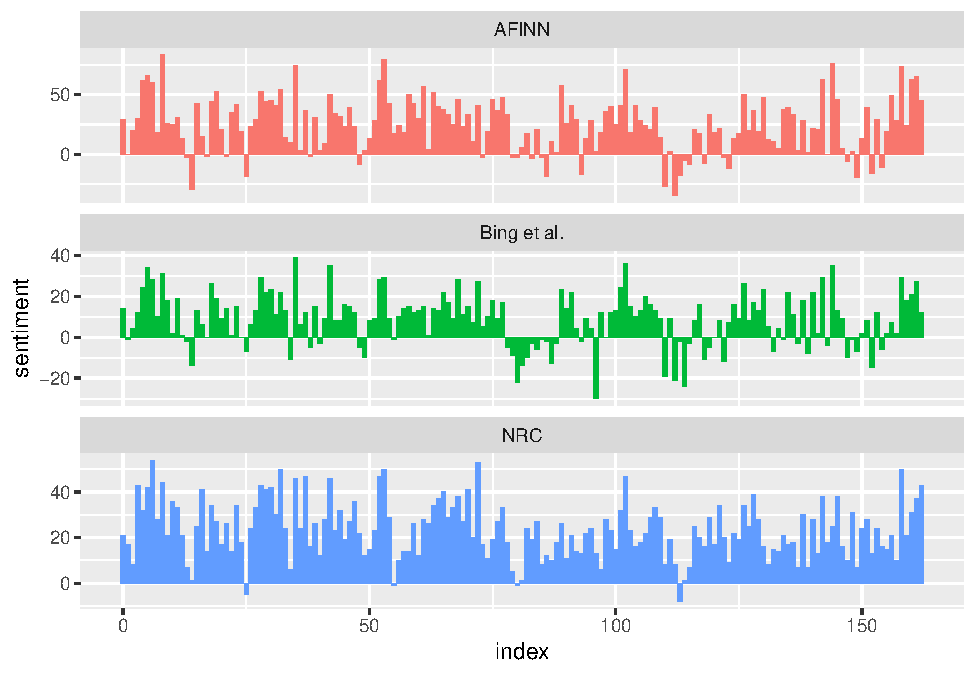
\includegraphics{Final_Project_files/figure-latex/unnamed-chunk-6-1.pdf}

The trend is nearly identical to that of the total emissions in figure 1
as its points have only been spread out to accommodate each month within
the year. In this case, our study year of 2020 on the far right of the
figure. The spacing is small but there are seven points above this year
with variation in how they lay. Importantly, the reduction in emissions
from average is clearly visible as the point drop below the magnitude of
any other values. These few points correspond to the peak in
restrictions on travel and businesses. We can break the months out
further, selecting only the year of 2020.

\begin{Shaded}
\begin{Highlighting}[]
\NormalTok{source}\FloatTok{.2020} \OperatorTok\StringTok{ }
\StringTok{  }\KeywordTok{filter}\NormalTok{(Column_Order }\OperatorTok{==}\StringTok{ }\DecValTok{14}\NormalTok{) }\OperatorTok\StringTok{ }
\StringTok{  }\KeywordTok{ggplot}\NormalTok{(}\KeywordTok{aes}\NormalTok{(YYYYMM, Value)) }\OperatorTok{+}\StringTok{ }
\StringTok{  }\KeywordTok{geom_point}\NormalTok{(}\KeywordTok{aes}\NormalTok{(}\DataTypeTok{color =}\NormalTok{ Description)) }\OperatorTok{+}\StringTok{ }
\StringTok{  }\KeywordTok{geom_smooth}\NormalTok{() }\OperatorTok{+}\StringTok{ }
\StringTok{  }\KeywordTok{geom_hline}\NormalTok{(}\DataTypeTok{yintercept =}\NormalTok{ est.co2}\OperatorTok{$}\NormalTok{obs}\FloatTok{.1973}\OperatorTok{/}\DecValTok{12}\NormalTok{, }\DataTypeTok{color =} \StringTok{"blue"}\NormalTok{, }\DataTypeTok{linetype =} \StringTok{"dashed"}\NormalTok{)  }\OperatorTok{+}
\StringTok{  }\KeywordTok{geom_hline}\NormalTok{(}\DataTypeTok{yintercept =}\NormalTok{ est.co2}\OperatorTok{$}\NormalTok{est}\FloatTok{.2020}\OperatorTok{/}\DecValTok{12}\NormalTok{, }\DataTypeTok{color =} \StringTok{"dark green"}\NormalTok{, }\DataTypeTok{linetype =} \StringTok{"dotdash"}\NormalTok{, }\DataTypeTok{size =} \DecValTok{1}\NormalTok{) }\OperatorTok{+}
\StringTok{    }\KeywordTok{labs}\NormalTok{(}\DataTypeTok{x =} \StringTok{"Time"}\NormalTok{, }
       \DataTypeTok{y =} \StringTok{"Million Metric Tons CO2"}\NormalTok{, }
       \DataTypeTok{title =} \StringTok{"Total CO2 Emissions in US in 2020"}\NormalTok{, }
       \DataTypeTok{subtitle =} \StringTok{"Using Monthly Totals from All Energy Sources"}\NormalTok{, }
       \DataTypeTok{caption =} \StringTok{"Figure 3"}\NormalTok{) }\OperatorTok{+}\StringTok{ }
\StringTok{  }\KeywordTok{theme_classic}\NormalTok{() }\OperatorTok{+}\StringTok{ }
\StringTok{  }\KeywordTok{theme}\NormalTok{(}\DataTypeTok{plot.title =} \KeywordTok{element_text}\NormalTok{(}\DataTypeTok{hjust =} \FloatTok{0.5}\NormalTok{),}
        \DataTypeTok{plot.subtitle =} \KeywordTok{element_text}\NormalTok{(}\DataTypeTok{hjust =} \FloatTok{0.5}\NormalTok{), }
        \DataTypeTok{legend.position =} \StringTok{"none"}\NormalTok{,}
        \DataTypeTok{plot.caption =} \KeywordTok{element_text}\NormalTok{(}\DataTypeTok{hjust =} \FloatTok{0.5}\NormalTok{))}
\end{Highlighting}
\end{Shaded}

\begin{verbatim}
## `geom_smooth()` using method = 'loess' and formula 'y ~ x'
\end{verbatim}

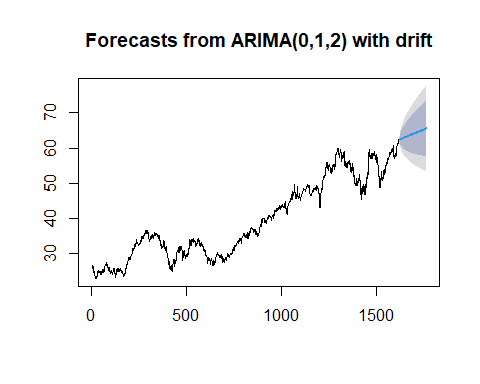
\includegraphics{Final_Project_files/figure-latex/unnamed-chunk-7-1.pdf}

From this point of view, it is much easier to see the drop in emissions
below the normal, or blue line of average monthly emissions total from
1973 through 2019. Even if the upper bounding of the loess smoothing
error range were the true values, the likelihood of the average monthly
emissions meeting the average months from previous years (at least for
these first 7 months) appears unlikely. The depth of the valley created
by the dark blue trendline appears too deep to allow emissions to creep
up and out of it as the points currently sit. This is good news for
mitigation of climate change.

Unfortunately, there is a worrying pattern that might be cause for
concern, from an emissions standpoint. The data appear to be rebounding
towards higher emissions for June and July. This could be from the
easing of restrictions and rebounding of individuals traveling. We have
already proven with reasonable confidence that this decrease in
emissions was not a natural variation. However, a large disease outbreak
has only been known to occur around once every hundred years; for
example, the Spanish flu epidemic in 1918. Given that our study covers a
little less than half of a century, we would not be able to visibly see
these changes because there are little to no comprehensive emissions
records in the U.S. during that time. Instead, it is possible to review
how energy is consumed and produced.

\begin{Shaded}
\begin{Highlighting}[]
\NormalTok{sector }\OperatorTok\StringTok{ }
\StringTok{  }\KeywordTok{filter}\NormalTok{(Column_Order }\OperatorTok{==}\StringTok{ "11"}\NormalTok{) }\OperatorTok
\StringTok{  }\KeywordTok{filter}\NormalTok{(Value }\OperatorTok{<}\StringTok{ }\DecValTok{20000}\NormalTok{) }\OperatorTok\StringTok{ }
\StringTok{  }\KeywordTok{ggplot}\NormalTok{(}\KeywordTok{aes}\NormalTok{ (YYYYMM, Value)) }\OperatorTok{+}\StringTok{ }
\StringTok{  }\KeywordTok{geom_point}\NormalTok{(}\KeywordTok{aes}\NormalTok{(}\DataTypeTok{color =}\NormalTok{ Description)) }\OperatorTok{+}\StringTok{ }
\StringTok{  }\KeywordTok{geom_smooth}\NormalTok{(}\DataTypeTok{method =} \StringTok{"lm"}\NormalTok{, }\KeywordTok{aes}\NormalTok{(}\DataTypeTok{color =} \StringTok{"Linear Trend"}\NormalTok{)) }\OperatorTok{+}\StringTok{ }
\StringTok{  }\KeywordTok{geom_smooth}\NormalTok{() }\OperatorTok{+}
\StringTok{   }\KeywordTok{labs}\NormalTok{(}\DataTypeTok{x =} \StringTok{"Time"}\NormalTok{, }
       \DataTypeTok{y =} \StringTok{"Trillion Btu"}\NormalTok{, }
       \DataTypeTok{title =} \StringTok{"Total Primary Energy Consumed in US"}\NormalTok{, }
       \DataTypeTok{subtitle =} \StringTok{"Using Monthly Totals from All Energy Sectors"}\NormalTok{, }
       \DataTypeTok{caption =} \StringTok{"Figure 4"}\NormalTok{) }\OperatorTok{+}\StringTok{ }
\StringTok{  }\KeywordTok{theme_classic}\NormalTok{() }\OperatorTok{+}\StringTok{ }
\StringTok{  }\KeywordTok{theme}\NormalTok{(}\DataTypeTok{plot.title =} \KeywordTok{element_text}\NormalTok{(}\DataTypeTok{hjust =} \FloatTok{0.5}\NormalTok{),}
        \DataTypeTok{plot.subtitle =} \KeywordTok{element_text}\NormalTok{(}\DataTypeTok{hjust =} \FloatTok{0.5}\NormalTok{),}
        \DataTypeTok{plot.caption =} \KeywordTok{element_text}\NormalTok{(}\DataTypeTok{hjust =} \FloatTok{0.5}\NormalTok{),}
        \DataTypeTok{legend.position =} \StringTok{"top"}\NormalTok{) }
\end{Highlighting}
\end{Shaded}

\begin{verbatim}
## `geom_smooth()` using formula 'y ~ x'
\end{verbatim}

\begin{verbatim}
## `geom_smooth()` using method = 'loess' and formula 'y ~ x'
\end{verbatim}

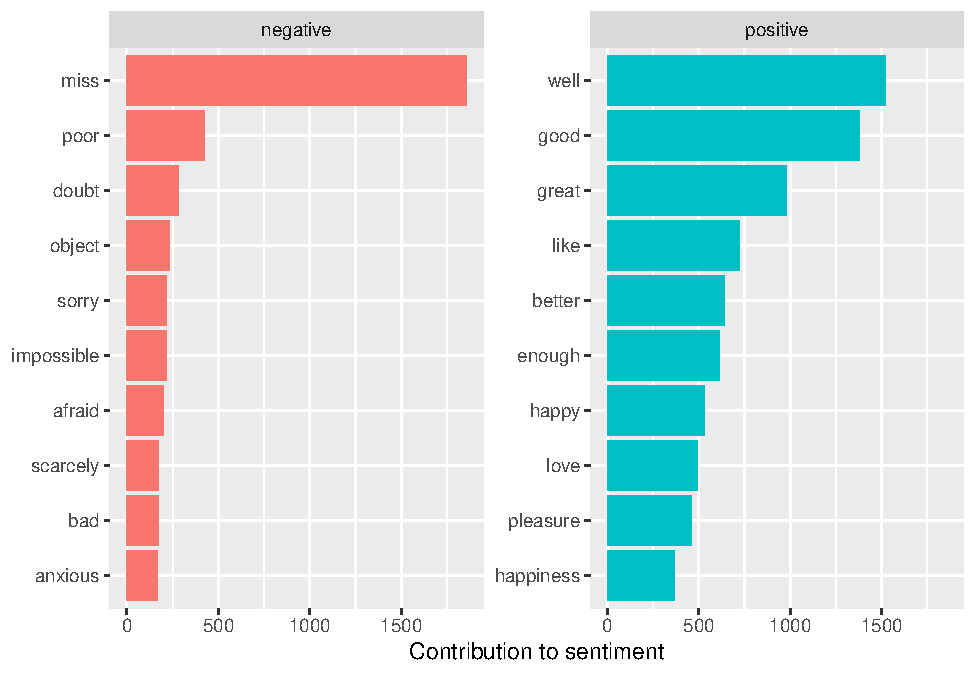
\includegraphics{Final_Project_files/figure-latex/unnamed-chunk-8-1.pdf}

The straight red line is a linear line of best fit for the monthly
emission totals. The curvy blue line depicts the consumption of primary
energy using a loess line. Although the red line is not the best fit, it
is easier to see the positive increase in energy consumption over time
which is still rooted in the data. The loess also shows this but it
seems to indicate a slightly decreasing trend in energy consumption from
2000 until present. Notice also, energy consumption for 2020 is much
lower than the surrounding points. Energy consumption appears it would
be correlated with the emissions of carbon dioxide quite well in this
chart.

\begin{Shaded}
\begin{Highlighting}[]
\NormalTok{producer }\OperatorTok\StringTok{ }
\StringTok{  }\KeywordTok{filter}\NormalTok{(Column_Order }\OperatorTok{==}\StringTok{ "1"}\NormalTok{) }\OperatorTok\StringTok{ }
\StringTok{  }\KeywordTok{filter}\NormalTok{(Value }\OperatorTok{<}\StringTok{ }\DecValTok{20}\NormalTok{) }\OperatorTok\StringTok{ }
\StringTok{  }\KeywordTok{ggplot}\NormalTok{(}\KeywordTok{aes}\NormalTok{(YYYYMM, Value)) }\OperatorTok{+}\StringTok{ }
\StringTok{  }\KeywordTok{geom_point}\NormalTok{(}\KeywordTok{aes}\NormalTok{(}\DataTypeTok{color =}\NormalTok{ Description)) }\OperatorTok{+}
\StringTok{  }\KeywordTok{geom_smooth}\NormalTok{() }\OperatorTok{+}
\StringTok{   }\KeywordTok{labs}\NormalTok{(}\DataTypeTok{x =} \StringTok{"Time"}\NormalTok{, }
       \DataTypeTok{y =} \StringTok{"Quad Btu"}\NormalTok{, }
       \DataTypeTok{title =} \StringTok{"Total Fossil Fuel Production in US"}\NormalTok{, }
       \DataTypeTok{subtitle =} \StringTok{"Using Monthly Energy Totals from Burning Fossil Fuels"}\NormalTok{, }
       \DataTypeTok{caption =} \StringTok{"Figure 5"}\NormalTok{) }\OperatorTok{+}\StringTok{ }
\StringTok{  }\KeywordTok{theme_classic}\NormalTok{() }\OperatorTok{+}\StringTok{ }
\StringTok{  }\KeywordTok{theme}\NormalTok{(}\DataTypeTok{plot.title =} \KeywordTok{element_text}\NormalTok{(}\DataTypeTok{hjust =} \FloatTok{0.5}\NormalTok{),}
        \DataTypeTok{plot.subtitle =} \KeywordTok{element_text}\NormalTok{(}\DataTypeTok{hjust =} \FloatTok{0.5}\NormalTok{),}
        \DataTypeTok{plot.caption =} \KeywordTok{element_text}\NormalTok{(}\DataTypeTok{hjust =} \FloatTok{0.5}\NormalTok{),}
        \DataTypeTok{legend.position =} \StringTok{"none"}\NormalTok{) }
\end{Highlighting}
\end{Shaded}

\begin{verbatim}
## `geom_smooth()` using method = 'loess' and formula 'y ~ x'
\end{verbatim}

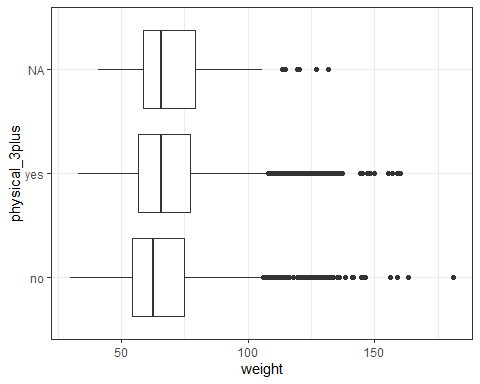
\includegraphics{Final_Project_files/figure-latex/unnamed-chunk-9-1.pdf}

Perhaps the most clear pattern in this figure is the evidence of a rapid
increase in fossil fuel production starting a little before 2010. The
reason for this is unknown and upon closer inspection there has been a
slightly increasing trend since the start of the study in 1973. 2020
remains an abnormality although, from the perspective of fossil fuel
burning for energy, there was another drop in production sometime
between 2013 and 2018 and it does not follow the rapid upward production
trend. A small decrease around 1998 and 1999 also seems tiny compared to
the larger much steep slope of the multiple quadrillion british thermal
units generated after 2010. A review of renewable energy data may help
shed some light on the reason for this pattern.

\begin{Shaded}
\begin{Highlighting}[]
\NormalTok{producer }\OperatorTok\StringTok{ }
\StringTok{  }\KeywordTok{filter}\NormalTok{(Column_Order }\OperatorTok{==}\StringTok{ "3"}\NormalTok{) }\OperatorTok\StringTok{ }
\StringTok{  }\KeywordTok{filter}\NormalTok{(Value }\OperatorTok{<}\StringTok{ }\DecValTok{2}\NormalTok{) }\OperatorTok\StringTok{ }
\StringTok{  }\KeywordTok{ggplot}\NormalTok{(}\KeywordTok{aes}\NormalTok{(YYYYMM, Value)) }\OperatorTok{+}\StringTok{ }\KeywordTok{geom_point}\NormalTok{(}\KeywordTok{aes}\NormalTok{(}\DataTypeTok{color =}\NormalTok{ Description)) }\OperatorTok{+}
\StringTok{   }\KeywordTok{geom_smooth}\NormalTok{() }\OperatorTok{+}
\StringTok{   }\KeywordTok{labs}\NormalTok{(}\DataTypeTok{x =} \StringTok{"Time"}\NormalTok{, }
       \DataTypeTok{y =} \StringTok{"Quad Btu"}\NormalTok{, }
       \DataTypeTok{title =} \StringTok{"Total Renewable Energy Production in US"}\NormalTok{, }
       \DataTypeTok{subtitle =} \StringTok{"Using Monthly Energy Totals from Renewable Sourcs"}\NormalTok{, }
       \DataTypeTok{caption =} \StringTok{"Figure 6"}\NormalTok{) }\OperatorTok{+}\StringTok{ }
\StringTok{  }\KeywordTok{theme_classic}\NormalTok{() }\OperatorTok{+}\StringTok{ }
\StringTok{  }\KeywordTok{theme}\NormalTok{(}\DataTypeTok{plot.title =} \KeywordTok{element_text}\NormalTok{(}\DataTypeTok{hjust =} \FloatTok{0.5}\NormalTok{),}
        \DataTypeTok{plot.subtitle =} \KeywordTok{element_text}\NormalTok{(}\DataTypeTok{hjust =} \FloatTok{0.5}\NormalTok{), }
        \DataTypeTok{legend.position =} \StringTok{"none"}\NormalTok{) }
\end{Highlighting}
\end{Shaded}

\begin{verbatim}
## `geom_smooth()` using method = 'loess' and formula 'y ~ x'
\end{verbatim}

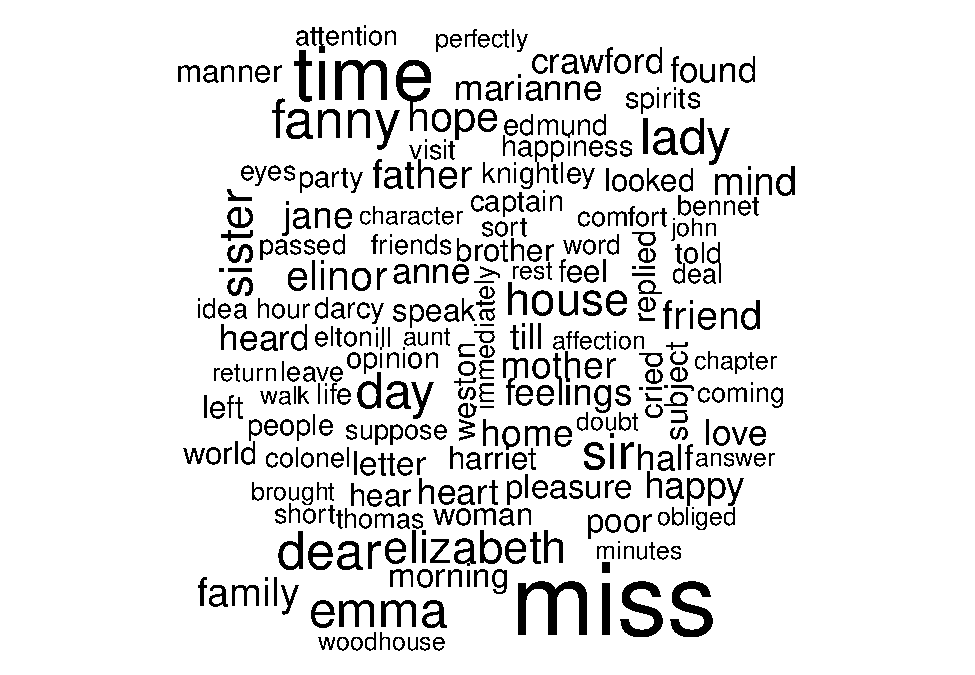
\includegraphics{Final_Project_files/figure-latex/unnamed-chunk-10-1.pdf}

While there is greater variation within the points, the level of
magnitude is four times smaller than fossil fuel production, though the
trend is increasing rapidly as well. Interestingly, there is no evidence
of a drop in 2020, as shown in previous figures on fossil fuel
production, energy consumption, and carbon dioxide emissions. This
factor is unique by comparison suggesting that renewable sources of
energy might be more resilient in times of crisis, strictly with respect
to disease outbreaks based on our current variables.

Determining the major sources of carbon dioxide emissions could also
increase the evidence in support of the significance of our study year's
variation from normal. Since this is primarily for visual inference as
it has already been proven statistically significant, we review the top
4 largest emitters for the duration of the study. A line chart was
chosen for this purpose in figure 7.

\begin{Shaded}
\begin{Highlighting}[]
\CommentTok{# Largest 4 sources of emission - everything else is below 1000 }
\NormalTok{source }\OperatorTok\StringTok{ }
\StringTok{  }\KeywordTok{subset}\NormalTok{(Column_Order }\OperatorTok{==}\StringTok{ }\KeywordTok{c}\NormalTok{(}\DecValTok{1}\NormalTok{,}\DecValTok{2}\NormalTok{,}\DecValTok{13}\NormalTok{,}\DecValTok{9}\NormalTok{)) }\OperatorTok\StringTok{ }
\StringTok{  }\KeywordTok{ggplot}\NormalTok{(}\KeywordTok{aes}\NormalTok{(YYYYMM, Value)) }\OperatorTok{+}\StringTok{ }
\StringTok{  }\KeywordTok{geom_line}\NormalTok{(}\KeywordTok{aes}\NormalTok{(}\DataTypeTok{color =}\NormalTok{ MSN)) }\OperatorTok{+}\StringTok{ }
\StringTok{  }\KeywordTok{geom_point}\NormalTok{(}\KeywordTok{aes}\NormalTok{(}\DataTypeTok{color=}\NormalTok{MSN)) }\OperatorTok{+}
\StringTok{    }\KeywordTok{labs}\NormalTok{(}\DataTypeTok{x =} \StringTok{"Time"}\NormalTok{, }
       \DataTypeTok{y =} \StringTok{"Million Metric Tons CO2"}\NormalTok{, }
       \DataTypeTok{title =} \StringTok{"Total CO2 Emissions in US"}\NormalTok{, }
       \DataTypeTok{subtitle =} \StringTok{"Using Yearly Totals from Each Energy Sources"}\NormalTok{,}
       \DataTypeTok{caption =} \StringTok{"Figure 7"}\NormalTok{) }\OperatorTok{+}\StringTok{ }
\StringTok{  }\KeywordTok{theme_classic}\NormalTok{() }\OperatorTok{+}\StringTok{ }
\StringTok{  }\KeywordTok{theme}\NormalTok{(}\DataTypeTok{plot.title =} \KeywordTok{element_text}\NormalTok{(}\DataTypeTok{hjust =} \FloatTok{0.5}\NormalTok{),}
        \DataTypeTok{plot.subtitle =} \KeywordTok{element_text}\NormalTok{(}\DataTypeTok{hjust =} \FloatTok{0.5}\NormalTok{), }
        \DataTypeTok{legend.position =} \StringTok{"top"}\NormalTok{, }
        \DataTypeTok{plot.caption =} \KeywordTok{element_text}\NormalTok{(}\DataTypeTok{hjust =} \FloatTok{0.5}\NormalTok{)) }
\end{Highlighting}
\end{Shaded}

\begin{verbatim}
## Warning in Column_Order == c(1, 2, 13, 9): longer object length is not a
## multiple of shorter object length
\end{verbatim}

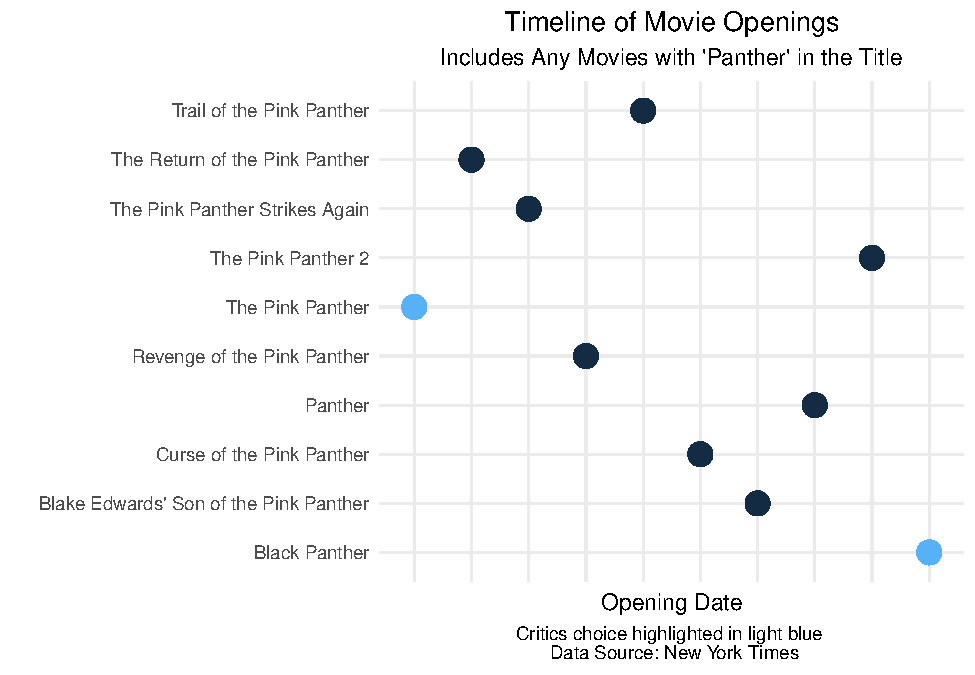
\includegraphics{Final_Project_files/figure-latex/unnamed-chunk-11-1.pdf}

Mnemonic series names are used for labeling and translate to the carbon
dioxide emissions from coal (including coal coke net imports) in purple,
natural gas (excluding supplemental gaseous fuels) in light blue, motor
gasoline (excluding ethanol) in red, and petroleum (excluding biofuels)
in green. There is a switch leading emitting sources as coal (in red)
has been decreasing quickly since about 2008. This made room for the
growth of natural gas and the swap of leadership between the two
occurred in the mid 2010's. In the following five years, going through
the months of our 2020 study year, coal encountered a greater decline
resulting in another brief change in leadership then reversal in 2020.
This time, gasoline is narrowly behind in 2020 while it appears it would
have sustained itself comfortably ahead based on prior patterns.

Current conditions imposed on emission sources appear to cause those
emission sources to reshuffle. So too, is the production of energy. We
review the current trends in a bar chart of each available producer type
in this data set. Each color corresponds to a new production category
and the energy they produce is measured in quadrillion british thermal
units.

\begin{Shaded}
\begin{Highlighting}[]
\KeywordTok{ggplot}\NormalTok{(producer, }\KeywordTok{aes}\NormalTok{(Description, Value)) }\OperatorTok{+}\StringTok{ }
\StringTok{  }\KeywordTok{geom_col}\NormalTok{(}\KeywordTok{aes}\NormalTok{(}\DataTypeTok{fill =}\NormalTok{ Description)) }\OperatorTok{+}\StringTok{ }
\StringTok{  }\KeywordTok{labs}\NormalTok{(}\DataTypeTok{x =} \StringTok{"Category"}\NormalTok{, }
       \DataTypeTok{y =} \StringTok{"Quad Btu"}\NormalTok{, }
       \DataTypeTok{title =} \StringTok{"Energy Production in US"}\NormalTok{, }
       \DataTypeTok{subtitle =} \StringTok{"Categorized by Types of Producers"}\NormalTok{, }
       \DataTypeTok{caption =} \StringTok{"Figure 8"}\NormalTok{)}\OperatorTok{+}\StringTok{ }
\StringTok{  }\KeywordTok{theme_classic}\NormalTok{() }\OperatorTok{+}\StringTok{ }
\StringTok{  }\KeywordTok{theme}\NormalTok{(}\DataTypeTok{plot.title =} \KeywordTok{element_text}\NormalTok{(}\DataTypeTok{hjust =} \FloatTok{0.5}\NormalTok{),}
        \DataTypeTok{plot.subtitle =} \KeywordTok{element_text}\NormalTok{(}\DataTypeTok{hjust =} \FloatTok{0.5}\NormalTok{),}
        \DataTypeTok{plot.caption =} \KeywordTok{element_text}\NormalTok{(}\DataTypeTok{hjust =} \FloatTok{0.5}\NormalTok{),}
        \DataTypeTok{legend.position =} \StringTok{"right"}\NormalTok{, }
        \DataTypeTok{axis.text =} \KeywordTok{element_blank}\NormalTok{()) }
\end{Highlighting}
\end{Shaded}

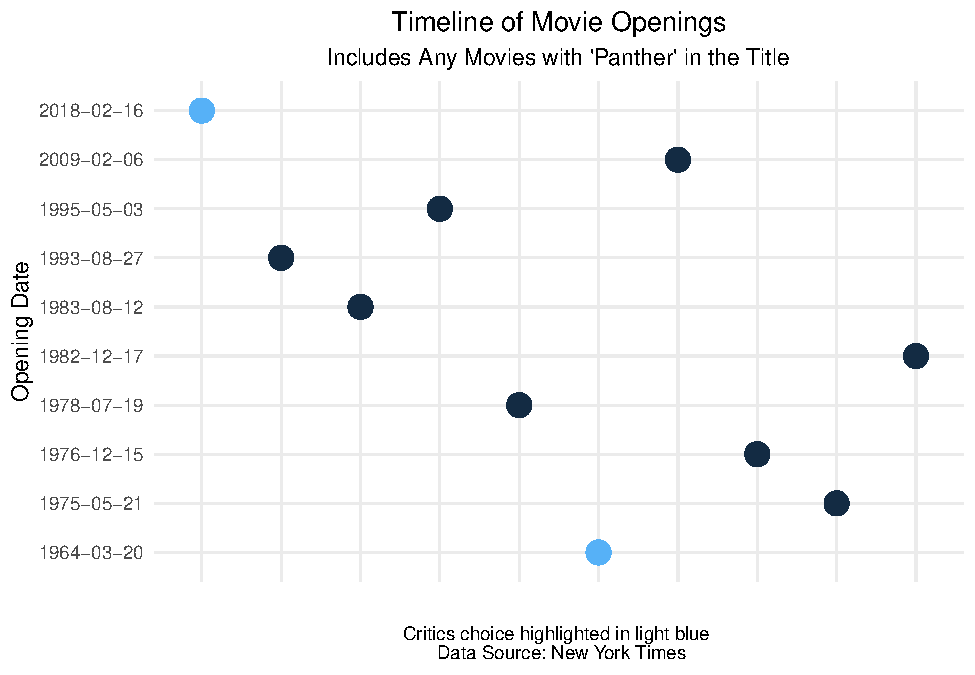
\includegraphics{Final_Project_files/figure-latex/unnamed-chunk-12-1.pdf}

By far, the dominant source of energy production in the U.S. is fossil
fuels. These bars are shown in the center of the chart on figure 8
directly adjacent the total primary energy consumption and production
bars. In terms of shear size, they easily make up more than 75\% of the
total primary energy production and total primary energy consumption. We
do produce less energy than demanded for consumption purposes relying on
imports of energy to make up the difference of this energy gap.

\begin{Shaded}
\begin{Highlighting}[]
\NormalTok{producer }\OperatorTok\StringTok{ }
\StringTok{  }\KeywordTok{filter}\NormalTok{(Column_Order }\OperatorTok{==}\StringTok{ }\KeywordTok{c}\NormalTok{(}\DecValTok{1}\NormalTok{,}\DecValTok{9}\NormalTok{,}\DecValTok{3}\NormalTok{,}\DecValTok{11}\NormalTok{,}\DecValTok{2}\NormalTok{,}\DecValTok{10}\NormalTok{)) }\OperatorTok
\KeywordTok{ggplot}\NormalTok{(}\KeywordTok{aes}\NormalTok{(Description, Value)) }\OperatorTok{+}\StringTok{ }
\StringTok{  }\KeywordTok{geom_boxplot}\NormalTok{(}\KeywordTok{aes}\NormalTok{(}\DataTypeTok{color =}\NormalTok{ Description)) }\OperatorTok{+}\StringTok{ }
\StringTok{    }\KeywordTok{labs}\NormalTok{(}\DataTypeTok{x =} \StringTok{"Category"}\NormalTok{, }
       \DataTypeTok{y =} \StringTok{"Quad Btu"}\NormalTok{, }
       \DataTypeTok{title =} \StringTok{"Distribution of Energy Production in US"}\NormalTok{, }
       \DataTypeTok{subtitle =} \StringTok{"Categorized by Types of Producers"}\NormalTok{, }
       \DataTypeTok{caption =} \StringTok{"Figure 8"}\NormalTok{)}\OperatorTok{+}\StringTok{ }
\StringTok{  }\KeywordTok{theme_classic}\NormalTok{() }\OperatorTok{+}\StringTok{ }
\StringTok{  }\KeywordTok{theme}\NormalTok{(}\DataTypeTok{plot.title =} \KeywordTok{element_text}\NormalTok{(}\DataTypeTok{hjust =} \FloatTok{0.5}\NormalTok{),}
        \DataTypeTok{plot.subtitle =} \KeywordTok{element_text}\NormalTok{(}\DataTypeTok{hjust =} \FloatTok{0.5}\NormalTok{),}
        \DataTypeTok{plot.caption =} \KeywordTok{element_text}\NormalTok{(}\DataTypeTok{hjust =} \FloatTok{0.5}\NormalTok{),}
        \DataTypeTok{legend.position =} \StringTok{"right"}\NormalTok{, }
        \DataTypeTok{axis.text =} \KeywordTok{element_blank}\NormalTok{()) }\OperatorTok{+}\StringTok{ }
\StringTok{  }\KeywordTok{coord_flip}\NormalTok{()}
\end{Highlighting}
\end{Shaded}

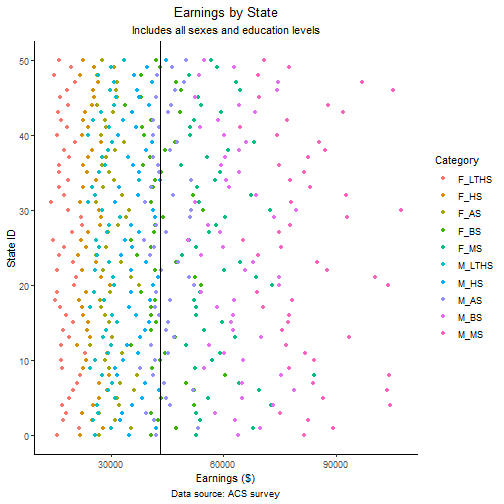
\includegraphics{Final_Project_files/figure-latex/unnamed-chunk-13-1.pdf}

Breaking down the production of energy from three main sources, we see
the distribution of fossil fuel production and consumption is far
greater in magnitude than either nuclear or renewable sources. Their
distribution is also much more evenly spread and centered about its
mean. The other sources, nuclear and renewable, have much smaller
ranges, less uniformity, and do not appear centered about their means.
Interestingly, fossil fuel production appears to make frequent attempts
at much greater production capacities while nuclear and renewable
sources remain stable in their production and consumption distribution.

\hypertarget{conclusion}{%
\subsection{Conclusion}\label{conclusion}}

In the time the United States was experiencing an unprecedented change
in the behavior of society due to the SARS-CoV-2 pandemic significant
reductions in carbon dioxide emissions were made. Normal emissions were
calculated to be 5,203.19 million metric tonnes of carbon dioxide
equivalent and the difference of 696.3399787 between the normal amount
and the estimated total of 2020 was significant at an alpha level of
0.05 with a p-value of 0.0269. The estimated total carbon dioxide for
2020 if the average monthly emissions remained at or near the average
for the last five months of August through December is 4506.85. This
would mean a reduction of about 73.24. However, this is not likely to
happen.

Given recent projections from the Energy Information Administration, it
is likely that emissions for the last five months will be greater than
the lowest points of the pandemic, regardless of travel or business
restrictions. This does not mean that emissions will balance themselves
out and suddenly result in average monthly emission standards. It is
highly probable that the total emissions for 2020 will be significantly
lower than the average of the previous two decades. This is good news
for climate change mitigation.

Current emission levels as of 2019 would almost equate to those of 1996.
A positive side-effect of this change in lifestyle would be a decrease
in transportation-related energy emissions, especially from motor
gasoline and similar petroleum products. This could lead to cleaner air,
less vehicular accidents, near-zero minute commute times, and the
associated health benefits that accompany reduction of vehicular
traffic. Keep in mind, this is only one aspect of the decrease in
emissions.

In addition to motor gasoline, we also noticed reductions in other
fossil fuels such as coal, including its coke net imports, aviation
fuel, and other petroleum products which make up 3 of the 4 largest
sources of emissions from carbon dioxide. From an emissions perspective,
these reductions are necessary to keep the average global temperatures
below 1.5 degrees Celsius of warming. The Intergovernmental Panel on
Climate Change (IPCC) predicts we need massive widespread changes in
nearly all aspects of our society if we are to avoid the worst aspects
of climate change.

If we were to attempt to maintain accordance with the Paris Climate
Agreement, we would need to maintain net-zero carbon emission by 2030.
For us to meet that goal from the study year further reductions are
necessary. Assuming the level in 2020 is estimated to be correct with a
significant reduction in carbon dioxide to a level of 4506.85 mmtco2e
and we can maintain it, then we would then need to cut emissions further
by another 500.7611111 mmtco2e per year for the remaining 9 years. This
has not happened in any year from our study.

The lowest annual emission amount since 1973 was 4,371 mmtco2e and it
occurred in 1983. For reference, the average monthly emissions then were
about 364.22 mmtco2e. That is already 11.35 mmtco2e lower than the
average emissions while on travel restrictions or mandatory quarantine
for portions of the year. Achieving the goals set by the Paris Climate
Agreement to avoid the worst of climate change, will require greater
change in energy production, sector consumption, and further reduction
of carbon dioxide emissions.

\hypertarget{references}{%
\subsection{References}\label{references}}

Brown, S., Nicholls, R. J., Goodwin, P., Haigh, I. D., Lincke, D.,
Vafeidis, A. T., Hinkel, J. (2018). Quantifying Land and People Exposed
to Sea-Level Rise with No Mitigation and 1.5°C and 2.0°C Rise in Global
Temperatures to Year 2300. Earth's Future, 6(3), 583-600.
\url{doi:10.1002/2017ef000738}

Goodwin, P., Brown, S., Haigh, I. D., Nicholls, R. J., Matter, J. M.
(2018). Adjusting Mitigation Pathways to Stabilize Climate at 1.5°C and
2.0°C Rise in Global Temperatures to Year 2300. Earth's Future, 6(3),
601-615. \url{doi:10.1002/2017ef000732}

Hausfather, Z. (2013). Explaining and Understanding Declines in U.S. CO2
Emissions. Retrieved from
\url{https://static.berkeleyearth.org/memos/explaining-declines-in-us-carbon.pdf}

IPCC, 2018: Global Warming of 1.5°C.An IPCC Special Report on the
impacts of global warming of 1.5°C above pre-industrial levels and
related global greenhouse gas emission pathways, in the context of
strengthening the global response to the threat of climate change,
sustainable development, and efforts to eradicate poverty.
{[}Masson-Delmotte, V., P. Zhai, H.-O. Pörtner, D. Roberts, J. Skea,
P.R. Shukla, A. Pirani, W. Moufouma-Okia, C. Péan, R. Pidcock, S.
Connors, J.B.R. Matthews, Y. Chen, X. Zhou, M.I. Gomis, E. Lonnoy, T.
Maycock, M. Tignor, and T. Waterfield (eds.){]}
\url{https://www.ipcc.ch/site/assets/uploads/sites/2/2019/06/SR15_Full_Report_High_Res.pdf}

Levin, K. (2018, October 10). 8 Things You Need to Know About the IPCC
1.5˚C Report. Retrieved December 05, 2020, from
\url{https://www.wri.org/blog/2018/10/8-things-you-need-know-about-ipcc-15-c-report}

Pielke, R. (2019, October 28). The World Is Not Going To Halve Carbon
Emissions By 2030, So Now What? Retrieved from
\url{https://www.forbes.com/sites/rogerpielke/2019/10/27/the-world-is-not-going-to-reduce-carbon-dioxide-emissions-by-50-by-2030-now-what/?sh=218f62eb3794}

Tracy, S. (2020, May 15). Global Lockdown for All - Except Carbon
Emissions. Retrieved December 05, 2020, from
\url{http://sitn.hms.harvard.edu/flash/2020/global-lockdown-for-all-except-carbon-emissions/}

USGS. (2018). How much carbon dioxide does the United States and the
World emit each year from energy sources? Retrieved from
\url{https://www.usgs.gov/faqs/how-much-carbon-dioxide-does-united-states-and-world-emit-each-year-energy-sources?qt-news_science_products=0}

United Nations. (2015, December 12). Paris Climate Agreement: Framework
Convention on Climate Change. Retrieved from
\url{https://assets.documentcloud.org/documents/2646274/Updated-l09r01.pdf}

\end{document}
